\section{Data access}
The data can be downloaded and accessed via the Copernicus Climate Change Service (C3S) Climate Data Store (CDS) Date:
\begin{center}
\sloppy\url{https://cds.copernicus-climate.eu/cdsapp\#!/dataset/in-situ-observations-surface-marine?tab=form}.
 \end{center}
The page has 3 tabs, the Overview tab presents an overview of the marine data and provides details on the data description, main and related variables available, contact email and links to licence/data policy statements. 
The Documentation tab provides links to PDF’s of the Marine Product User Guide, Marine data inventories, Common Data Model specifications and a link to the Data Deposit Server webpage. The Download Data tab provides 6 sections that need to be completed in order to download data. The first selects one or more variables (Figure \ref{fig:cds_variable_main}) from the available ECVs (Table \ref{tab:ecvs}). The second selects the level of quality control to apply, selecting either those that have passed all stages of quality control or all observations (Figure \ref{fig:cds_qc_main}). The next three select the time period  by selecting the year (Figure \ref{fig:cds_year_main}), month (Figure \ref{fig:cds_month_main}) and day (Figure \ref{fig:cds_day_main}). The final selection selects the region, specifying either select all data (global) or observation within a bounding box (Figure \ref{fig:cds_area_main}).

Data can additionally be downloaded using the CDS Python API. Selecting the \texttt{Show API request} button reveals the API commands to use for the given selection (Figure \ref{fig:cds_api_main}). More information can be found at:

\begin{center}
\url{https://cds.climate.copernicus.eu/api-how-to}
\end{center}

\begin{figure}[h]
\begin{center}
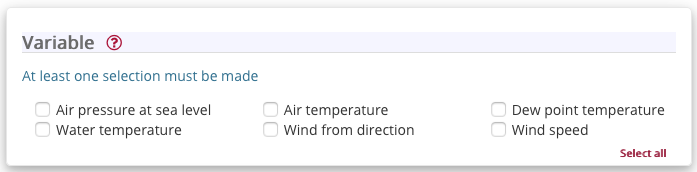
\includegraphics[width=0.75\textwidth]{resources/cds_variable_select.png}
\caption{Selection box for variable selection on the Global Land And Marine Observations Database download page on the CDS.}
\label{fig:cds_variable_main}
\end{center}
\end{figure}


\begin{figure}
\begin{center}
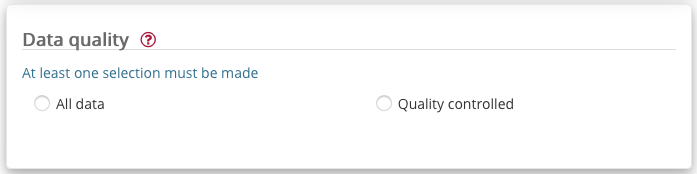
\includegraphics[width=0.75\textwidth]{resources/cds_qc_select.png}
\caption{Selection box for quality status on the Global Land And Marine Observations Database download page on the CDS.}
\label{fig:cds_qc_main}
\end{center}
\end{figure}

\begin{figure}
\begin{center}
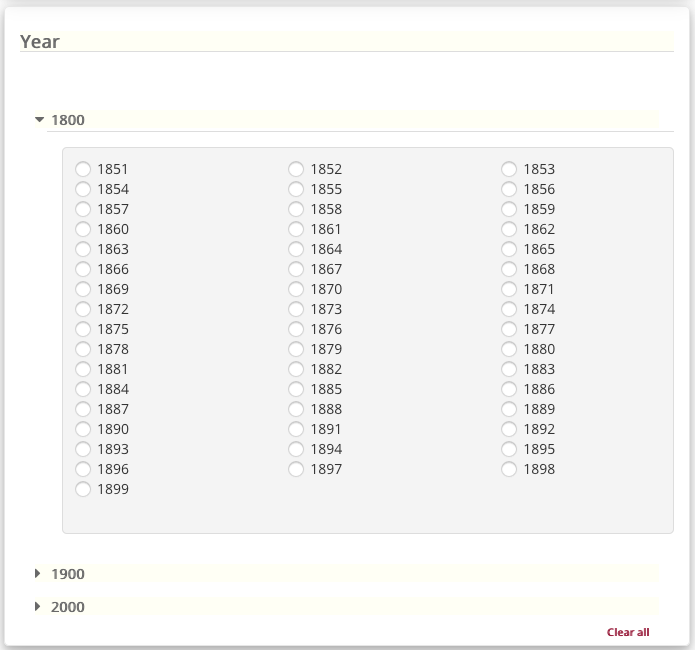
\includegraphics[width=0.75\textwidth]{resources/cds_year_select.png}
\caption{Selection box for selecting year on the Global Land And Marine Observations Database download page on the CDS.}
\label{fig:cds_year_main}
\end{center}
\end{figure}

\begin{figure}
\begin{center}
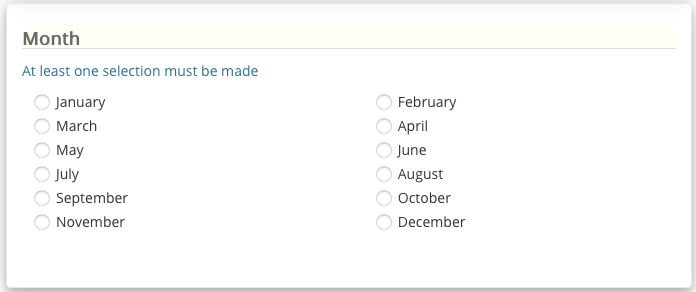
\includegraphics[width=0.75\textwidth]{resources/cds_month_select.png}
\caption{Selection box for selecting month on the Global Land And Marine Observations Database download page on the CDS.}
\label{fig:cds_month_main}
\end{center}
\end{figure}

\begin{figure}
\begin{center}
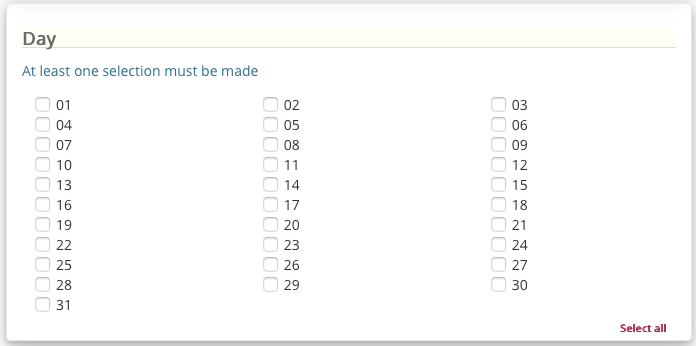
\includegraphics[width=0.75\textwidth]{resources/cds_day_select.png}
\caption{Selection box for selecting day on the Global Land And Marine Observations Database download page on the CDS.}
\label{fig:cds_day_main}
\end{center}
\end{figure}

\begin{figure}
\begin{center}
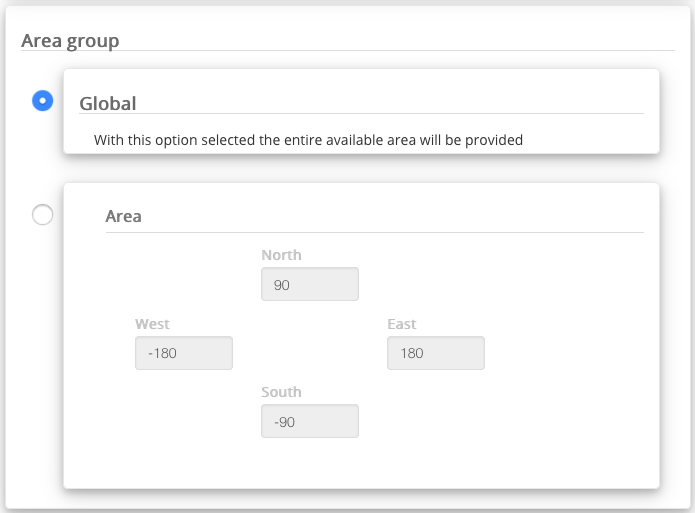
\includegraphics[width=0.75\textwidth]{resources/cds_area_select.png}
\caption{Selection box for selecting area on the Global Land And Marine Observations Database download page on the CDS.}
\label{fig:cds_area_main}
\end{center}
\end{figure}

\begin{figure}
\begin{center}
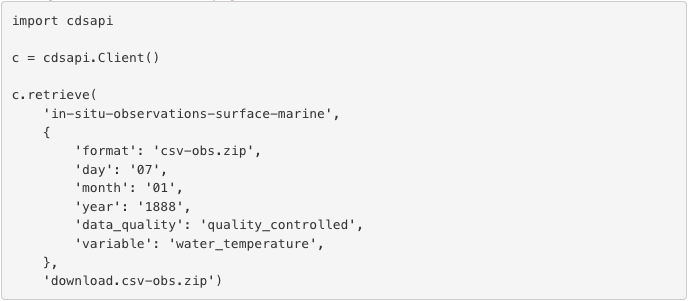
\includegraphics[width=0.75\textwidth]{resources/cds_api_request.png}
\caption{Example API request to download data from the Global Land And Marine Observations Database.}
\label{fig:cds_api_main}
\end{center}
\end{figure}
\FloatBarrier
